\section{Data processing}
\begin{frame}{Graph}
\center{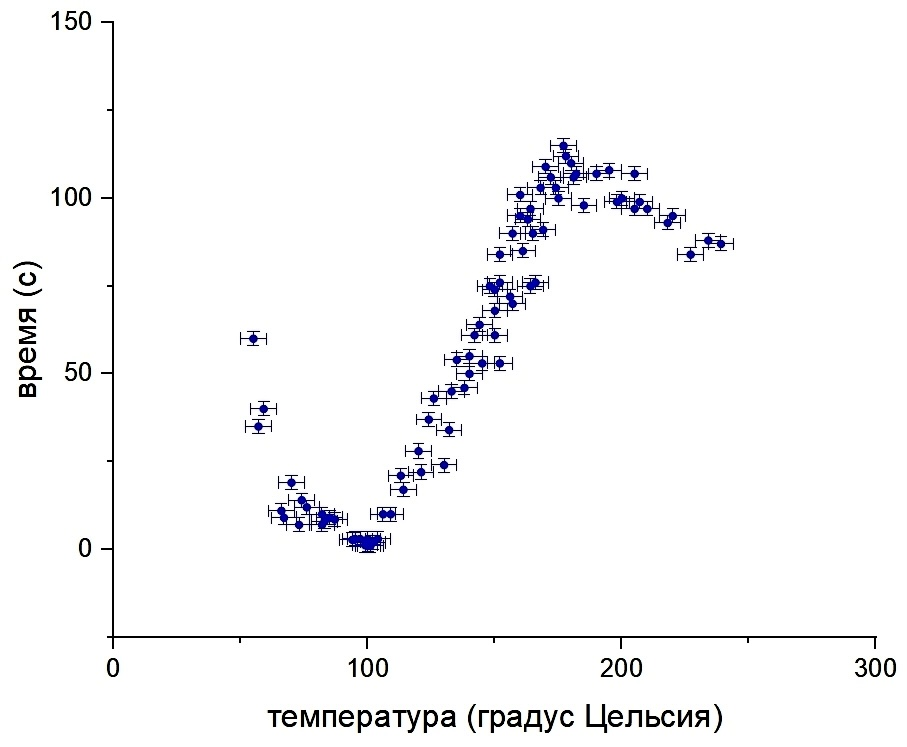
\includegraphics[scale = 0.28]{tex/conclusao/IMG_7656.jpg}}
\end{frame}

\begin{frame}{Graph approximation}
\center{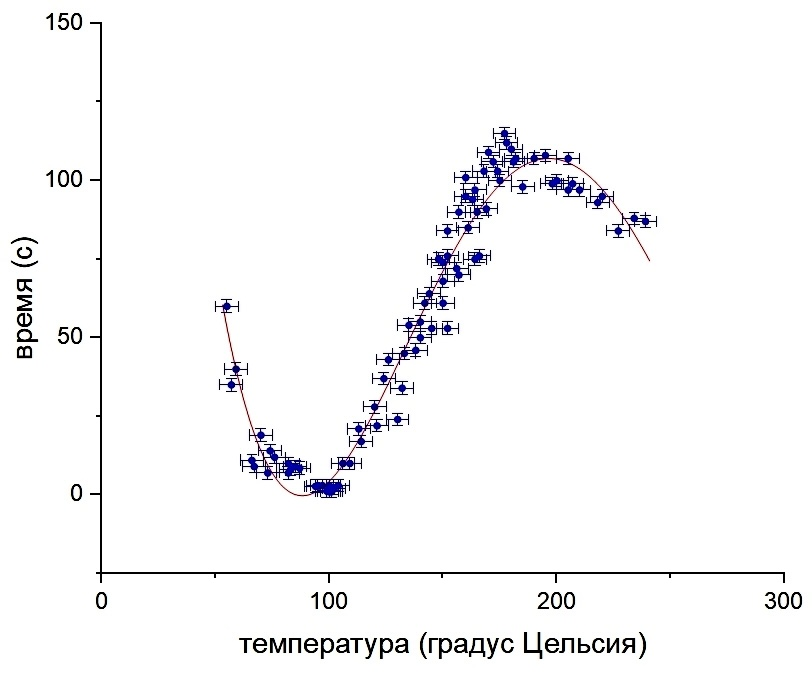
\includegraphics[scale = 0.3]{tex/conclusao/IMG_7596.jpg}}
\end{frame}
 \begin{frame}{Немного наблюдений, обнаруженных во время эксперемента}
  \begin{block}{Геометрия капли}
   После падения даже с небольшой высоты, у капли самовозбуждаются колебания, которые затухают без внешнего воздействия, с уменьшением размера капли. 
  \end{block}   
  \center{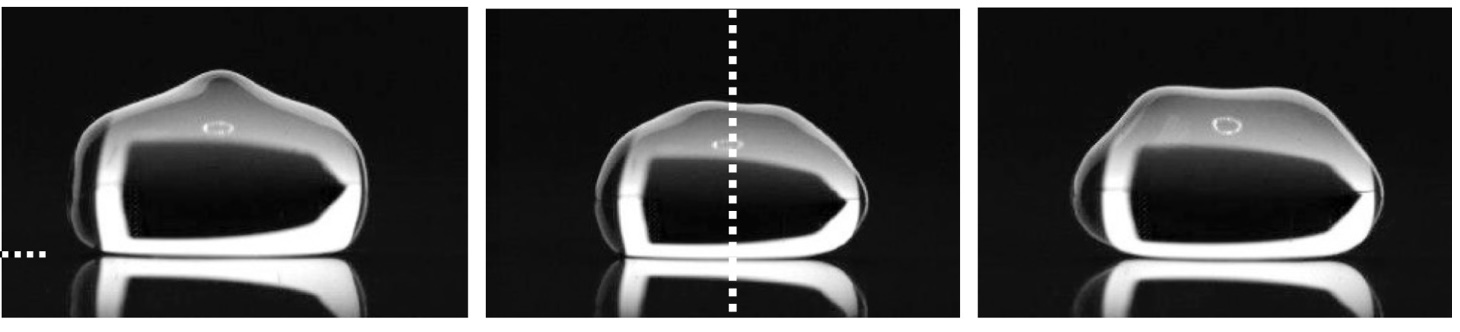
\includegraphics[scale = 0.2]{tex/conclusao/IMG_7594.jpg}}
  \begin{block}{}
      Такая нестабильность является обратной нестабильностью Рэлея-Тейлора, которая происходит, когда сила гравитации преобладает над поверхностным натяжением.
  \end{block}
 \end{frame}

\begin{frame}{}
  \begin{minipage}[h]{0.49\linewidth}
{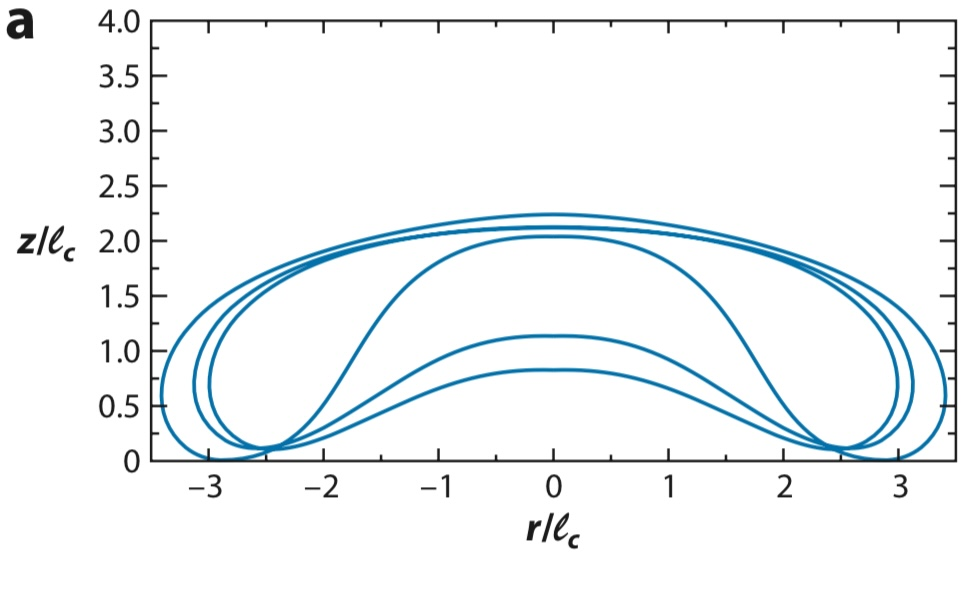
\includegraphics[width=\linewidth]{tex/conclusao/IMG_7593.jpg}}
\label{fig:image}
\end{minipage}
\begin{minipage}[h]{0.49\linewidth}
{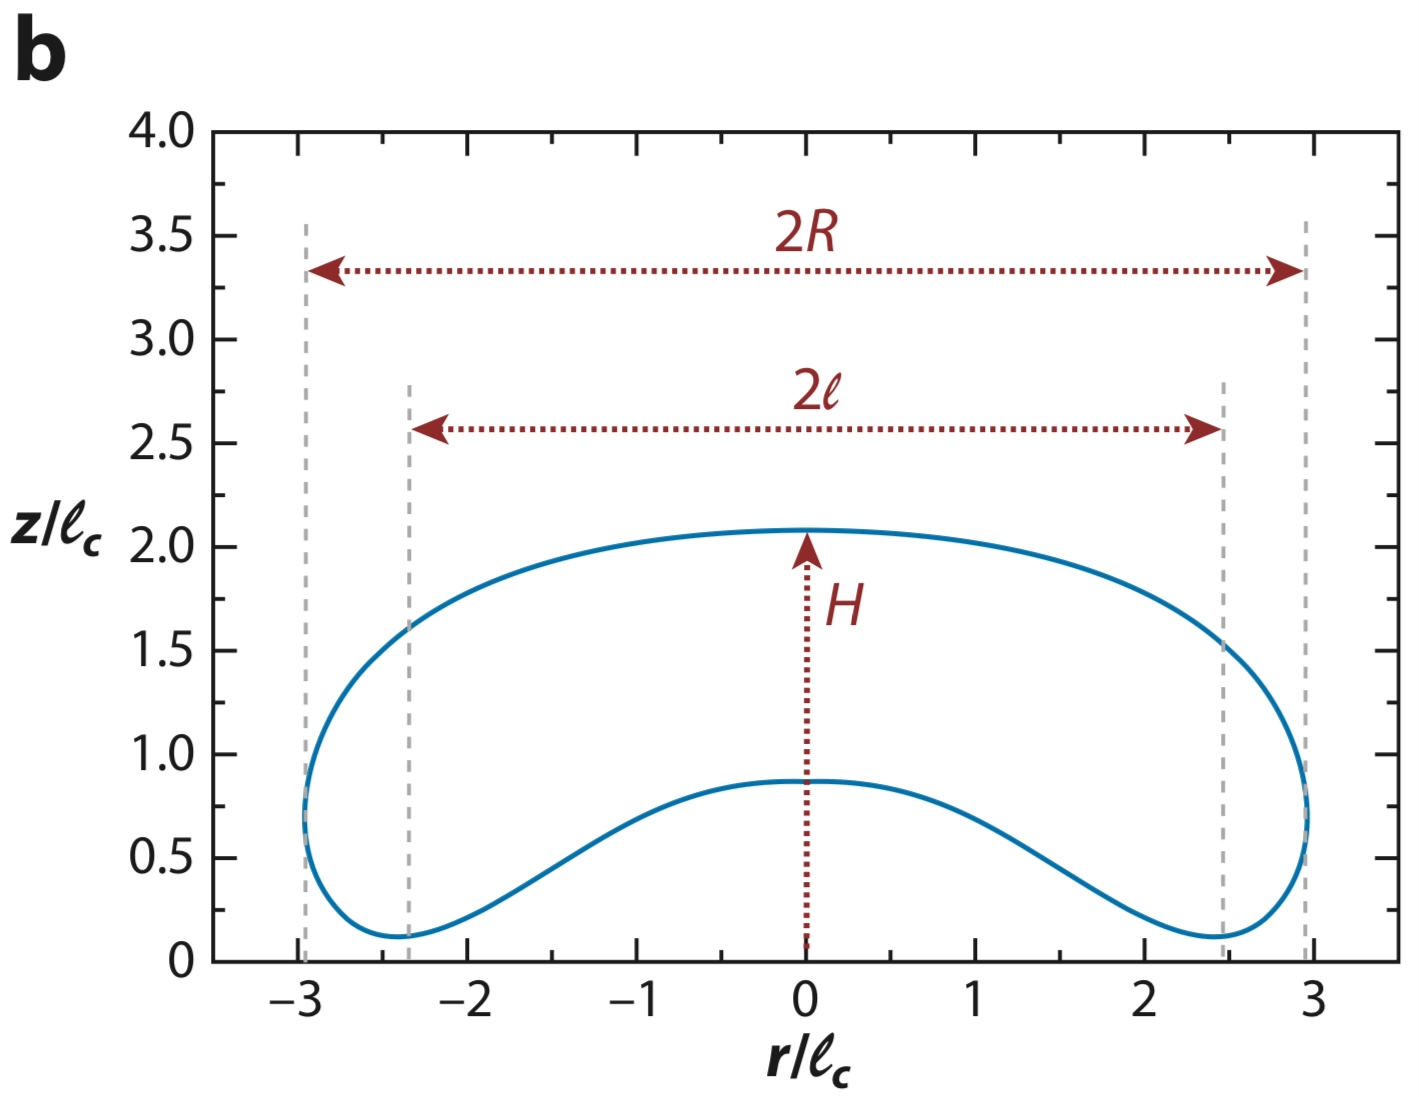
\includegraphics[width=\linewidth]{tex/conclusao/IMG_7592.jpg}}
\end{minipage}
\begin{block}{Зависимость от радиуса}
 Неравновесие сил происходит, когда радиус контакта \(\ell\) превышает порог \(\ell^{*} = 3\ell_{c}\), определяется, как длина капиляра, соответсвующий критический радиус \(R^{*}=4,3\ell_{c} \), где
 \({\ell_{c}=\left(\frac{\gamma}{\rho g}\right)}^{1/2}\), \(\gamma=59\ mN\ m^{-1}\), - коэфициент поверхностного \\
 \vspace{0.10cm}
 натяжения \(\ell_{c}=2,5 mm.\) для воды.
 \end{block}
\end{frame}

 \begin{frame}{}
 \vspace{0.2cm}
   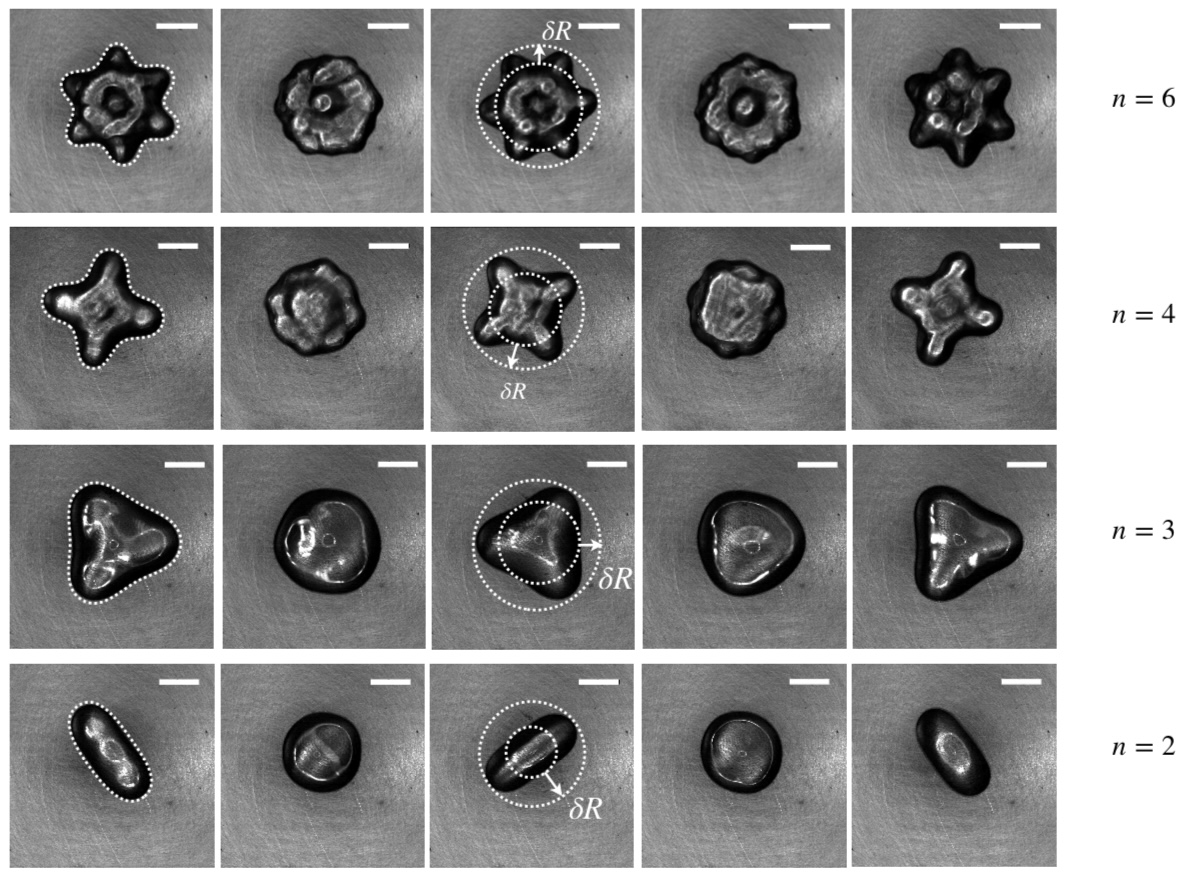
\includegraphics[width=\linewidth]{tex/conclusao/IMG_7598.jpg}
 \end{frame}
 \begin{frame}{}
 \vspace{1.5cm}
 \begin{block}{Как описать, явления на картинках, с разными рисунками, пр. разных n?}
 Осесиметричное сферическое падение подвергается свободным колебаниям на естественной резонансной частоте \(f_{n}\), где n - целые числа, в пределах малых деформаций задаётся уравнением:
 \[f_{n}= \frac{1}{2\pi}\sqrt{n\left(n-1\right)\left(n+2\right)}\sqrt{\frac{\gamma}{\rho R^{3}}}\]
  
 \end{block}
 \end{frame}